% Add common preamble to the document
%% This file is shared between thesis and proposal

\documentclass[a4paper,12pt,twoside]{report}

\usepackage[scaled]{helvet}
\usepackage{url}
\usepackage{cite}
\usepackage{listings}
\usepackage[pdftex]{graphicx}
\usepackage[hang,small,bf]{caption}
\usepackage{styles/tum}
\usepackage{setspace}
\usepackage[german,english]{babel}
\usepackage{float}
\usepackage{floatflt}
\usepackage{fancyhdr}
\usepackage{color}
\usepackage{booktabs}
\usepackage[pdftex,bookmarks=true,plainpages=false,pdfpagelabels=true]{hyperref}	%TODO make yourself familiar with \label, \ref and \hyperref for referencing figures, tables, chapters, etc.
\usepackage{mdwlist}
\usepackage{enumerate}
\usepackage{array}
\usepackage{longtable}
\usepackage[utf8]{inputenc}
\usepackage[capitalize, noabbrev]{cleveref}
\usepackage{wasysym}
\usepackage{todonotes}

% Path for graphics
\graphicspath{{figures/}}

% Include the Thesis metadata like title, author, etc. 
\input{metadata}

%%%%%%%%%%%%%%%%%%%%%%%%%%%%%%%%%%%%%%%%%%%%%%%%%%%%%%%%%%%%%%%%%%%%%%%%%%%%%%%%%%%%%%%%%%%%%%%%%
% Custom Commands for this template
%%%%%%%%%%%%%%%%%%%%%%%%%%%%%%%%%%%%%%%%%%%%%%%%%%%%%%%%%%%%%%%%%%%%%%%%%%%%%%%%%%%%%%%%%%%%%%%%%

% Annotate feedback you received 
\newcommand{\feedback}[1]{\todo[inline,color=green,caption={}]{#1}}

% State what is missing in this spot
\newcommand{\missing}[1]{\todo[inline,color=yellow,caption={}]{#1}}

% Inline to do note: 
\newcommand{\TODO}[1]{\todo[inline,caption={}]{#1}}





\def\proposal{Proposal for}

%%%%%%%%%%%%%%%%%%%%%%%%%%%%%%%%%%%%%%%%%%%%%%%%%%%%%%%%%%%
% Theses specific packages go here
%%%%%%%%%%%%%%%%%%%%%%%%%%%%%%%%%%%%%%%%%%%%%%%%%%%%%%%%%%%
\usepackage[nolist]{acronym}
\usepackage{csquotes}

%%%%%%%%%%%%%%%%%%%%%%%%%%%%%%%%%%%%%%%%%%%%%%%%%%%%%%%%%%%
% Begin of document
%%%%%%%%%%%%%%%%%%%%%%%%%%%%%%%%%%%%%%%%%%%%%%%%%%%%%%%%%%%
\begin{document}
\setlength{\evensidemargin}{22pt}
\setlength{\oddsidemargin}{22pt}


\hypersetup{pdfborder={0 0 0}, pdfauthor={\author}, pdftitle={\title}}

\lstset{showspaces=false, numbers=left, frame=single, basicstyle=\small}

%------- Title setup -------
\thispagestyle{empty}
{
\sffamily

\vspace{1cm}
\begin{center}
\oTUM{4cm}

\vspace{5mm}     
{\LARGE \bf \sffamily Technical University of Munich}

\vspace{5mm}
{\Large School of Computation, Information and Technology \\ -- Informatics -- }	
\vspace{1mm}
\end{center}

\vspace{15mm}

\begin{center}
        {\large {\proposal} {\degree}'s Thesis in \program}
\vspace{8mm}

\begin{spacing}{1.3}
{\LARGE \bf \sffamily \title}\\
\vspace{8mm}

{\LARGE \titleGer}\\
\vspace{8mm}
\end{spacing}

\begin{tabular}{ll}
\large Author:           & \large \author     \\[2mm]
\large Supervisor:       & \large \supervisor \\[2mm]				
\large Advisor:	         & \large \advisor    \\[2mm]
\ifx\proposal\empty\else
\large Start Date:       & \large \startdate  \\[2mm]
\fi
\large Submission Date:  & \large \date
\end{tabular}

\end{center}
}


\selectlanguage{english}
\pagenumbering{arabic}

\fancyhead{}
\pagestyle{fancy}
\fancyhead[LE]{\slshape \leftmark}
\fancyhead[RO]{\slshape \rightmark}
\headheight=15pt

%------- Start of Proposal -------
\section*{Introduction}
% - Introduce the reader to the general setting
% - What is the environment?
% - What are the tools in use?

The number of students in Computer Science courses at universities is increasing steadily. At the Technical University of Munich, the number of full-time students\footnote{i.e., full-time equivalents} has increased by more than 2,400 within five year recently~\cite{tumInZahlen2020}. This fact also means that the number of exercise submissions in Informatics courses has increased drastically.
These circumstances pose a problem for the instructors, as it is hard to give feedback to all students individually. There exist courses using automatically tested exercises, but those are often difficult to create and get right. Manually graded exercises can provide more individuality, but it is hard to give feedback to all students.

Artemis is an online learning platform for exercise management~\cite{ArTEMiS}. It is being developed at the Technical University of Munich and used by several other universities in Germany. 

\begin{figure}[ht]
    \centering
    \includegraphics[width=0.8\linewidth]{figures/proposal/coffe-uml-activity-diagram.pdf}
    \caption{UML Activity Diagram from~\cite{cofee}: Overview of the machine learning activities in Athene}
    \label{fig:coffeeUmlActivityDiagram}
\end{figure}

Athene, a system for automatically generating feedback on text exercises, is integrated into Artemis~\cite{cofee}. It works by essentially clustering submissions into groups using machine learning techniques and then choosing feedback from the same cluster. The actual steps in the feedback generation process can be seen in~\cref{fig:coffeeUmlActivityDiagram}. In detail, they are~\cite{cofee}:
\begin{itemize}
    \item \textbf{Segmentation} of the submission: Athene splits the submission into parts by topics, which are identified using the presence or absence of certain keywords.
    \item \textbf{Language Embedding} of the parts: Athene embeds the parts to a vector representation using a pre-trained ELMo language model~\cite{deepContextualizedWordRepresentations}.
    \item \textbf{Clustering} of the vector representations: Athene clusters the vector representations using the Hierarchical Density-Based Spatial Clustering algorithm~\cite{hdbsc}.
\end{itemize}

Each of these steps is currently performed by one microservice, all of which are written in Python and implement one approach to each of the steps.
In addition, there is a tracking service for logging the feedback generation process~\cite{atheneTracking} and a load balancer for distributing the load between the microservices~\cite{atheneLoadBalancer}.

\begin{figure}[ht]
    \centering
    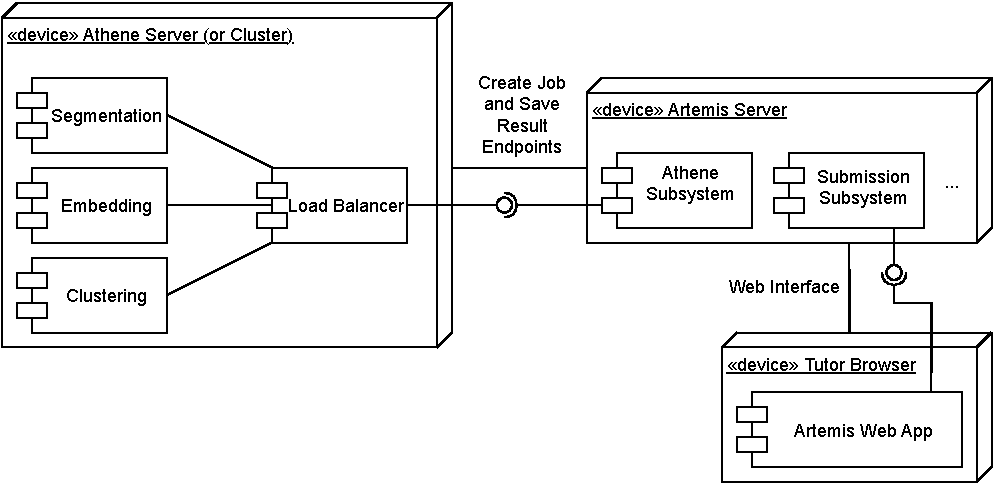
\includegraphics[width=0.8\linewidth]{figures/proposal/deployment-diagram.pdf}
    \caption{Rough overview of the current Athene and Artemis deployment setup: The \textit{Athene Subsystem} chooses feedback based on clusters sent by the \textit{Athene Server} after the feedback processing. Tutors later access those feedbacks via the \textit{Artemis Server}.}
    \label{fig:atheneArtemisDeployment}
\end{figure}

Currently, Athene sends a list of clusters and a list of segments to Artemis. Artemis then chooses feedbacks from the same cluster for the suggestions. The setup is also shown in~\cref{fig:atheneArtemisDeployment}.


\section*{Problem}
% - What is/are the problem(s)? 
% - Identify the actors and use these to describe how the problem negatively influences them.
% - Do not present solutions or alternatives yet!
% - Present the negative consequences in detail

Currently, Athene is bound to one approach for each step in the feedback generation process. This decreases the flexibility and extensibility of the system and should be improved.
On a more practical level, Athene does not support programming exercises, which are a common type of exercise in Computer Science courses.

Two types of actors could have problems with the current status of Athene:
\begin{itemize}
    \item \textbf{Tutors} in courses with manually graded programming exercises: They cannot profit from Athene's feedback generation capabilities, as Athene does not support programming exercises. This means that they won't get any automatically generated feedback suggestions for programming exercises, which would save them a lot of time.
    For textual exercises, Athene currently provides feedback suggestions for around 45\% of the submissions~\cite{cofee2}. This number might be improved even further in the future if the system is generalized to support different approaches for each step in the feedback generation process.
    \item It is difficult for \textbf{Developers} of Athene to integrate additional approaches and features into Athene, as the system is currently bound to one approach for each step in the feedback generation process. The choice of the feedback suggestion is also done by Artemis (outside of Athene), which makes it impossible to change the feedback suggestion independently of Artemis.
\end{itemize}

\section*{Motivation}
%- Outline why it is important to solve the problem
% - Again use the actors to present your solution, but don't be to specific
% - Be visionary! 
% - If applicable, motivate with existing research, previous work 

As student numbers will continue to rise (especially in Computer Science courses), the number of feedbacks which tutors have to give will increase as well. Extending Athene to support programming exercises would allow tutors to profit from its feedback generation capabilities and save them a lot of time.

Generalizing each of the steps in the feedback generation process would also allow developers to integrate additional approaches and features into Athene more easily.
For example, the clustering step could be replaced by a different clustering algorithm, which might improve the quality of the feedback suggestions. Past work like an evaluation of the helpfulness of feedbacks given by Athene~\cite{atheneTracking} or efforts to make it more language-independent~\cite{atheneLanguage} could also potentially have profited from more generalization.

Furthermore, groundwork on a more flexible system might enable relatively new innovations like ChatGPT to be used in Athene, if the feedback suggestion generation not only supports choosing existing feedbacks, but also generating new ones.

\section*{Objective}
% - What are the main goals of your thesis?
In the thesis, we want to enable Athene to support programming exercises and to generalize the steps in the feedback generation process. This should be done in a way that does not affect the current functionality of Athene and does not introduce any new bugs.

One of the advantages of having the possibility to choose dynamically between different ways of performing the steps in the feedback generation process is that it would allow us to switch them as necessary to implement feedback suggestions for programming exercises as well. 
As part of a project in the practical course \enquote{iPraktikum} at the Technical University of Munich, there already is a prototype for a system that can provide automatic feedback suggestions on programming exercises, called \enquote{ThemisML}\footnote{\url{https://github.com/ls1intum/Themis-ML}}. 
Parts of this system will be useful for integrating programming feedback suggestions into Athene. ThemisML uses codeBERT~\cite{codeBERT} to compute pairwise similarity scores between submissions to suggest appropriate feedback suggestions. We will evaluate a variety of approaches for effectively segmenting, embedding and clustering programming exercises to improve on the efficiency and quality of the feedback suggestions and to integrate them into Athene.

As automatic programming exercise feedback suggestions are not currently supported by Artemis, we also want to make those available in Artemis. Tutors should be able to accept or reject the suggestions in the web interface, similar to the existing automatic feedbacks on text exercises generated by Athene. Themis\footnote{\url{https://github.com/ls1intum/Themis}}, a new iPad app supporting grading of programming exercises, should also be able to use the programming feedback suggestions from Athene.

By moving the actual choice of feedbacks from Artemis to Athene, we want to make it possible to use change the feedback suggestion independently of Artemis. Also, Athene should offer a more general API: Currently, it computes the feedback clusters and sends them to Artemis in a ProtoBuf format. A fixed interface contract for the API would make it easier to integrate Athene into other systems.


\section*{Schedule}
% - When will the thesis Start (Always 15th of Month) 
% - Create a rough plan for your thesis (separate the time in sprints with a length of 2-4 Weeks)
% - Each sprint should contain several work items - Again keep it high-level and make to keep your plan realistic
% - Make sure the work-items are measurable and deliverable 
% - No writing related tasks! (e.g. "Write Analysis Chapter")

The following schedule roughly outlines the work items for the thesis.

\begin{itemize}
    \item \textbf{Generalize} the existing microservices for segmentation, embedding and clustering in Athene: It should be possible to easily switch between internal modules.
    \item \textbf{Move the actual choice of feedbacks} from Artemis to a new microservice within Athene: It should offer more general API endpoints for storing submissions, for storing feedbacks and for providing suggestions. Artemis should use these endpoints instead of the current ones.
    \item \textbf{Evaluate} different possibilities for segmenting, embedding and clustering programming exercises. Implement promising approaches and integrate them into Athene. % Maybe this should be first?
    \item Adding support for \textbf{programming exercises} in Athene:
    \begin{itemize}
        \item Add support for programming exercise segmentation, embedding and clustering as well as feedback suggestion generation to Athene
        \item Implement communication between Artemis and Athene for programming exercises into Artemis
        \item Add support for displaying automatic feedback suggestions for programming exercises in Artemis
    \end{itemize}
    \item \textbf{Integrate} feedback suggestions \textbf{into the Themis iPad app}: It should be able to display the programming feedback suggestions from Athene.
    \item Implement \textbf{improvements and bug fixes} still necessary for a stable release of Athene.
    \item Write \textbf{documentation and the thesis} for the project.
\end{itemize}


\clearpage
\begin{acronym}
\acro{GUI}{Graphical User Interface}
\end{acronym}

\clearpage
\bibliography{thesis}
\bibliographystyle{alpha}

\end{document}
